\section{\acf{XSS}}\label{sssec:XSSDefinition}

Der Quellcode einer Webseite besteht meistens aus drei Komponenten. Die Auszeichnungssprachen HTML und CSS sind dabei für die Struktur und das Aussehen der gelieferten Informationen zuständig. Der Webbrowser interpretiert die HTML-Elemente und erstellt darauf aufbauend das sogenannte \ac{DOM}. JavaScript, als dritte Komponente, kann zum Einen den Inhalt des DOM weiter bearbeiten und zum Anderen durch sogenannte Events weiteren Quellcode ausführen.

\subsection{Ziele von \ac{XSS}-Angriffen}
		Im wesentlichen werden XSS-Angriffe durchgeführt, um an sensible Daten des Opfers zu gelangen. Drei beispielhafte Ziele des Angreifers sind Diebstahl von \gls{Cookies}, Installieren eines \gls{Keylogger}s oder \gls{Phishing}.

		\begin{description}
			\item[Cookie-Diebstahl]{Durch den Diebstahl von Cookies kann sich der Angreifer als sein Opfer ausgeben, um sich Zugang zu der gewünschten Webseite zu verschaffen.}
			\item[Keylogger]{Der Angreifer kann einen Keylogger auf der Webseite einschleusen, um Benutzereingaben an den Server des Angreifers weiterzuleiten.}
			\item[Phishing]{Phishing beschreibt die Manipulation von Links oder Webseiten, sodass das Opfer auf eine gefälschte Webseite weitergeleitet wird. Gibt das Opfer dort seine Benutzerdaten ein, werden diese an den Angreifer geschickt.}
		\end{description}


\subsection{\ac{XSS}-Typen und Definitionen}
		Je nach Quelle des Angriffs wird \acl{XSS} in drei Arten unterschieden: 

		\begin{description}
			\item[Typ 0 / \acs{DOM}-basiertes \ac{XSS}] \ac{DOM}-basiertes XSS spielt sich komplett im Browser des Benutzers ab. Hierbei werden die Benutzereingaben nicht an die Webseite gesendet, sondern mittels JavaScript dazu verwendet, um das bestehende HTML-Dokument zu manipulieren.
			\item[Typ 1 / reflektiertes \ac{XSS}] Werden Benutzereingaben direkt in Form von Fehlermeldungen, Suchanfragen oder innerhalb der Webseite zurückgeliefert, kann reflektiertes \ac{XSS} auftreten.
			\item[Typ 2 / persistentes \ac{XSS}] Im Allgemeinen tritt persistentes \ac{XSS} auf, wenn der Payload auf dem angegriffenen Server, zum Beispiel in einer Datenbank, gespeichert wird. Durch Aufrufen der Seite zu einem späteren Zeitpunkt wird der Angriff geladen und ausgeführt.
		\end{description}
		
		In Abbildung \ref{fig:flowchartXSSType1} ist der Ablauf eines reflektierenden \ac{XSS}-Angriffs abgebildet, in dem der  Angreifer zunächst eine \ac{URL} mit bösartigen JavaScript-Quellcode erstellt. Diese \ac{URL} lässt der Angreifer vom Opfer aufrufen, sodass die Attacke von der Webseite verarbeitet und an den Browser vom Opfer ``reflektiert'' wird. Hierdurch wird der \ac{XSS}-Angriff beim Opfer ausgeführt.
		
		\begin{figure}[htbp] 
			\centering
			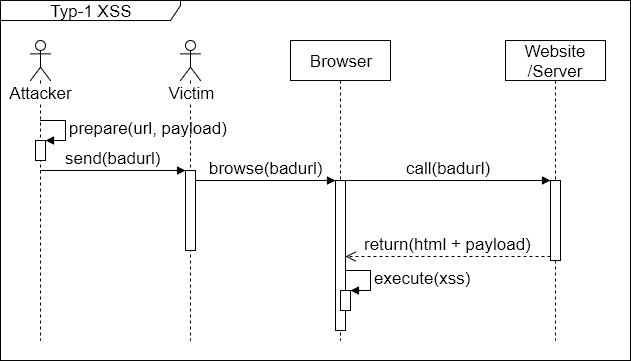
\includegraphics[width=\textwidth]{contents/images/FlowchartXSSType1}
			\caption{Ablaufdiagramm: Typ 1 XSS}
			\label{fig:flowchartXSSType1}
		\end{figure}
	
\FloatBarrier
		
		Im Gegensatz dazu ist in der Abbildung \ref{fig:flowchartXSSType2} exemplarisch der Ablauf eines persistenten \ac{XSS}-Angriffs (Typ 2) abgebildet. Hier gelingt es dem Angreifer, schädlichen JavaScript-Code in die Datenbank einer Webseite zu speichern. Dieser schädliche Code wird dann beim Laden der Webseite ausgeführt. Beispiele hierfür können Foren und Kommentarfunktionen sein. Das Opfer wird beim nächsten Aufruf der Seite unabsichtlich das Laden des bösartigen Quellcodes und somit die \ac{XSS}-Attacke auf dem Browser starten.
		
		\begin{figure}[htbp] 
			\centering
			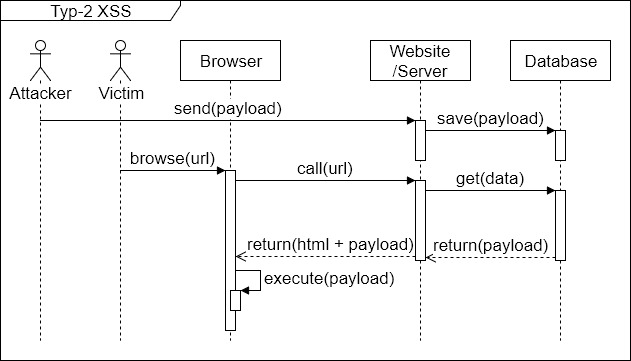
\includegraphics[width=\textwidth]{contents/images/FlowchartXSSType2}
			\caption{Ablaufdiagramm: Typ-2 XSS}
			\label{fig:flowchartXSSType2}
		\end{figure}
		
\FloatBarrier
			Seit Mitte 2012 hat sich in der Praxis eine neue Kategorisierung eingebürgert, da die bisherige Kategorisierung in Typ 0, Typ 1 und Typ 2 häufig für Verwirrung gesorgt hat. Grund hierfür ist, dass auch persistente und reflektierte \ac{XSS} außerhalb des \ac{DOM}-Kontextes auftreten können \cite{Wichers2017}.
		
%		Seit Mitte 2012 werden \ac{XSS}-Angriffe in zwei Kategorien unterteilt, um Verwirrung zu vermeiden, da auch Fälle von persistenten/reflektierenden nicht-DOM-\ac{XSS} auftreten können \cite{Wichers2017}. 
		
		\begin{description}
			\item [Server \ac{XSS}] Die gesamte Antwort (inklusive des Payloads) wird vom Server generiert und an den Browser gesendet. Dabei spielt es keine Rolle, ob der Payload aus der Datenbank oder einem Request stammt. Laut dieser Definition fallen die Beispiele \ref{fig:flowchartXSSType1} und \ref{fig:flowchartXSSType2} in die Server \ac{XSS} Klassifizierung, da bei beiden Angriffen der Payload im \ac{HTML}-Code an den Browser des Opfers geschickt wird.
			
			\item [Client \ac{XSS}] Der Angriff erfolgt ausschließlich im Browser des Opfers, das heißt, dass DOM ist bereits vom Server generiert und es findet kein weiterer Request mehr statt. 
			Auslöser des Payloads ist ein JavaScript-Methodenaufruf, welcher den Payload lädt und ausführt. Hier kann der Payload aus einem \gls{AJAX}-Aufruf oder dem \ac{DOM} stammen. 
		\end{description}

\subsection{Payloads}

\subsubsection{Aufbau eines Payloads}
		Ein Payload besteht im Kern aus einem Stück vom Angreifer bestimmten JavaScript-Quellcode. Hier kann theoret2aisch jede Funktion einprogrammiert werden. Für die Ermittlung der Schwachstelle reicht es jedoch aus, eine einfache alert-Box öffnen zu lassen. Dies kann in JavaScript mit den Methoden ``alert'', ``promt'' oder ``confirm'' erziehlt werden. In den folgenden Erklärungen wird \textbf{PAYLOAD} als generischer Platzhalter definiert und verwendet.

\subsubsection{Payload-Kontexte}
		
		Damit dieser Quelltext ausgeführt werden kann, muss sich der Methodenaufruf im JavaScript-Kontext befinden. Die direkte Einbindung von JavaScript in ein HTML-Dokument kann mittels des script-Tags erfolgen, wie in Quelltext \ref{lst:context-script-tag} dargestellt ist.
		
\begin{lstlisting}[language=HTML,caption={Kontexte: Payload in script-Tags},label=lst:context-script-tag]
<script>PAYLOAD</script>
<script src="path/to/myFile.js"></script> // Content: PAYLOAD
<script src="://url.to/myFile.js"></script> // Content: PAYLOAD
\end{lstlisting}
		
		Das script-Tag kann JavaScript-Quelltext entweder direkt enthalten oder zur Laufzeit mittels des src-Attributs einbinden. Der Inhalt der ``myFile.js''-Datei ist dementsprechend ebenfalls im JavaScript-Kontext. Wird der Payload innerhalb einer JavaScript-Methode (Quelltextbeispiel: \ref{lst:context-javascript-method}) eingesetzt, muss zunächst aus der Applikationslogik ausgebrochen werden.
		
\begin{lstlisting}[language=HTML,caption={Kontexte: Payload in Zuweisungswerten},label=lst:context-javascript-method]
<script> var a = "PAYLOAD"; </script>
\end{lstlisting}
		
		Wird der Payload direkt in den HTML-Quelltext eingesetzt, muss entweder ein künstlicher JavaScript-Kontext mittels des script-Tags oder eines Attributes erstellt werden. Die Platzierung des Payloads hängt hier von der Programmierung der Webseite ab. Es können hierbei wieder verschiedene Umgebungen identifiziert werden. Der einfachste Fall ist die Platzierung zwischen einem öffnenden und schließenden HTML-Tag, wie im Quelltextbeispiel \ref{lst:context-between-html-tag} dargestellt.
		
\begin{lstlisting}[language=HTML,caption={Kontexte: Payload zwischen HTML-Tags},label=lst:context-between-html-tag]
<div>PAYLOAD</div>
\end{lstlisting}
		
		Alternativ wären auch Attributnamen bzw. -werte oder HTML-Kommentare eine mögliche Umgebung, in der ein Payload eingefügt werden könnte. Die dazugehörigen Beispiele sind in Quelltext \ref{lst:context-comment-attributes} abgebildet.
		
\begin{lstlisting}[language=HTML,caption={Kontexte: Payload  in anderen Umgebungen},label=lst:context-comment-attributes]
<!-- PAYLOAD -->

<img src="path/to/image-PAYLOAD.jpg" />
<input onclick="PAYLOAD" />
<input PAYLOAD="This is some alt text." />
\end{lstlisting}
		
		Bei einer dynamischen Webseite werden oft Attribute von HTML-Elementen hinzugefügt, verändert oder entfernt. Ein Beispiel hierfür sind JavaScript-Bildergalerien, welche bei aktiven Bildern eine CSS-Klasse entfernen oder hinzufügen. Im Quelltextbeispiel \ref{lst:context-comment-attributes} Zeile 5 könnte eine Sicherheitslücke ausgenutzt werden, um den Payload anstatt des alt-Attributes in den HTML-Quellcode einzufügen.
		
\subsubsection{Kontextwechsel zu JavaScript}
		
		Nachdem die verschiedenen Umgebungen für eingefügte Payloads identifiziert worden sind, muss noch in den richtigen Kontext gewechselt werden. Dieser ist notwendig, da sonst der JavaScript-Interpreter den eingefügten Code nicht ausführen kann. Um dies zu erreichen, muss der Payload so erweitert werden, dass dieser den HTML-Kontext schließt und in den JavaScript-Kontext wechselt.
		
		Abbildung \ref{fig:PayloadContextSwitch} zeigt, wie ein solcher Payload inklusive Kontextwechsel aufgebaut sein kann. Hierbei wir der Platzhalter wird in dem gezeigten Beispiel durch einen dreiteiligen Payload ersetzt. Im ersten Teil schließt der Wert für das Value-Attribut ab und wechselt damit in den HTML-Kontext. Dieser Teil besteht i.d.R. nur aus wenigen Zeichen und wird unter anderem als ``Outbreak'' bezeichnet.  Der zweite Teil des Payloads erstellt ein neues Attribut innerhalb des Input-Tags und wechselt damit in den JavaScript-Kontext. Beim letzten Teil des Payloads wird der auszuführende JavaScript-Code eingefügt, der vom vorhandenen Rest des Input-Tags abgeschlossen wird.
		
		\begin{figure}[htbp] 
			\centering
			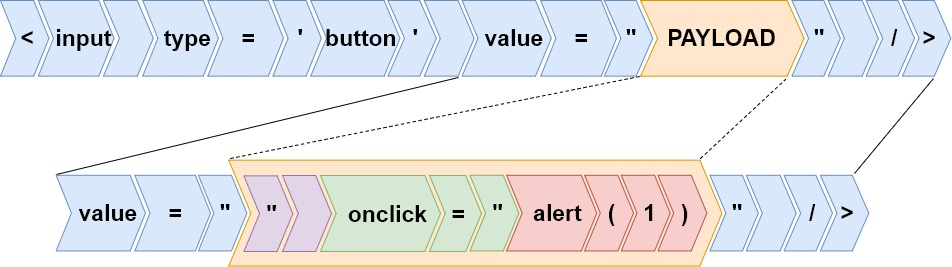
\includegraphics[width=\textwidth]{contents/images/PayloadContextSwitch}
			\caption{XSS-Beispiel: Kontextwechsel}
			\label{fig:PayloadContextSwitch}
		\end{figure}

\paragraph{Legende zu Abbildung \ref{fig:PayloadContextSwitch}}
		\begin{enumerate}
			\item[Blau] Ursprünglicher HTML-Code
			\item[Lila] Ausbruch aus dem aktuellen Kontext
			\item[Grün] Wechsel in den JavaScript-Kontext
			\item[Rot] Auszuführender JavaScript-Code
		\end{enumerate}
		
\subsection{Beispiele}
\subsubsection{\ac{XSS}-Angriff ohne Kontextwechsel}\label{ssec:example-without-context-change}
		Wie bereits in Quelltextbeispiel \ref{lst:context-javascript-method} und Zeile 4 des Quelltextbeispiels \ref{lst:context-comment-attributes} gezeigt, befinden sich die Payloads bereits in der richtigen Umgebung und werden beim Laden der Webseite ausgeführt.
		
\subsubsection{\ac{XSS}-Angriff mit Kontextwechsel}
		
		Um ein genaueres Verständnis vom Wechsel in den JavaScript-Kontext zu bekommen, wird im Folgenden das erste Level der Seite \url{https://xss-game.appspot.com/} betrachtet.
		
		Gegeben ist eine einfache HTML-Form mit einem Eingabefeld. Ziel ist es, aus dem HTML-Kontext, wie in der Abbildung \ref{fig:XSSGameLevelOneResponse} dargestellt, in den JavaScript-Kontext zu wechseln. Durch die Eingabe von \lstinline[language=html]!'><)(}{]["! lässt sich schnell ermitteln, ob wichtige Elemente von JavaScript herausgefiltert werden. 
		
		\begin{figure}[htbp] 
			\centering
			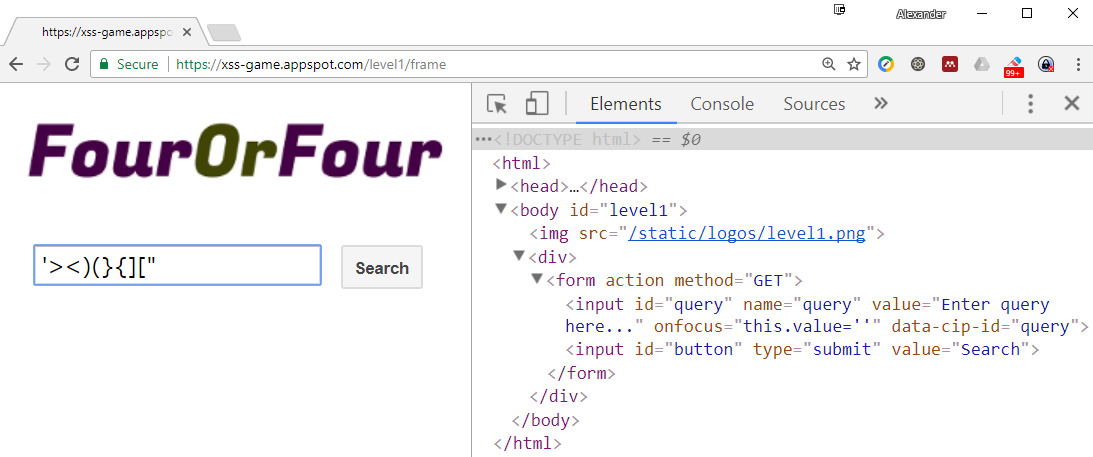
\includegraphics[width=0.80\textwidth]{contents/images/XSSGameLevelOneRequest}
			\caption{XSS-Game: Level 1 - Eingabemaske}
			\label{fig:XSSGameLevelOneRequest}
		\end{figure}
		
		Die Eingabe aus Abbildung \ref{fig:XSSGameLevelOneRequest} wird ohne Veränderung innerhalb des Bold-Tags \lstinline[language=html]!(<b></b>)! ausgegeben, was dem HTML-Kontext entspricht.
		
		\begin{figure}[htbp] 
			\centering	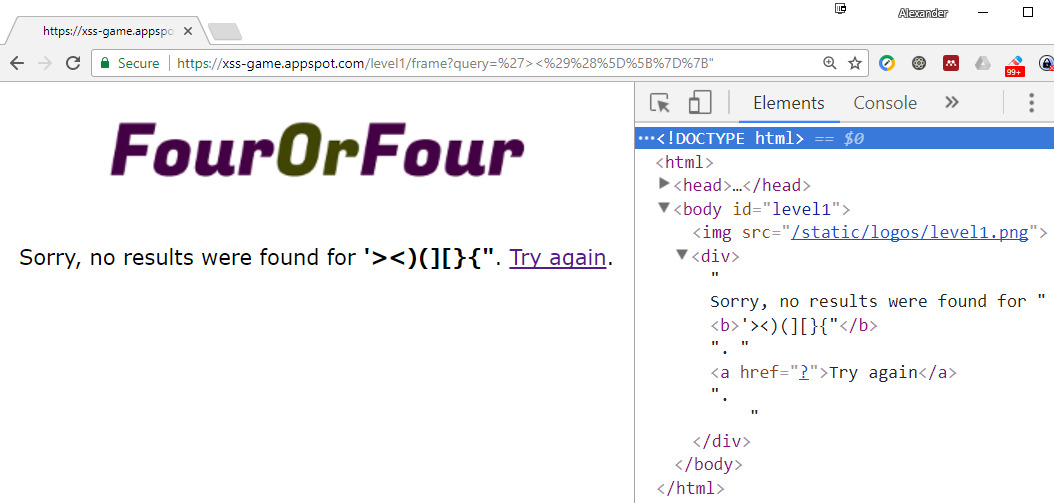
\includegraphics[width=0.80\textwidth]{contents/images/XSSGameLevelOneResponse}
			\caption{XSS-Game: Level 1 - Antwortseite}
			\label{fig:XSSGameLevelOneResponse}
		\end{figure}
\FloatBarrier
		Da die Webseite keinerlei Änderungen an der übergebenen Zeichenkette vornimmt, kann der Payload frei gewählt werden. Die gewählte Lösung für das obige Beispiel ist in Abbildung \ref{fig:XSSGameSolution} dargestellt. Im Gegensatz zur Abbildung \ref{fig:PayloadContextSwitch} ist hier keine Outbreak-Sequenz notwendig. Durch die umschließenden script-Tags kann der JavaScript-Kontext mit der Benutzereingabe definiert und übergeben werden.
		
		\begin{figure}[htbp] 
			\centering
			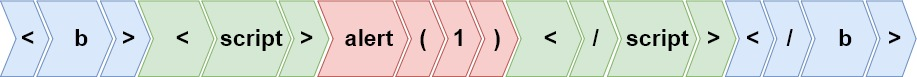
\includegraphics[width=\textwidth]{contents/images/XSSGameSolution}
			\caption{XSS-Game: Level 1 - Lösung}
			\label{fig:XSSGameSolution}
		\end{figure}

\FloatBarrier
\subsubsection{Ausführen des Payloads}
		
		Oft reicht das Einfügen im richtigen Kontext nicht aus, um die Ausführung zu starten. Wie in Quelltextbeispiel \ref{lst:example-javascript-context-onerror} dargestellt, wird die Payload-Zeichenkette bereits in den JavaScript-Kontext im onerror-Event eingefügt. Jedoch wird der eingefügte Code nicht ausgeführt, solange das Bild korrekt geladen werden kann.
		
\begin{lstlisting}[language=HTML,caption={XSS-Angriffe: ohne Kontextwechsel},label=lst:example-javascript-context-onerror]
<img src="path/to/image-1.jpg" onerror="PAYLOAD" />
\end{lstlisting}
		
		Die Lösung des Problems ist eine Veränderung der HTML-Komponenten des img-Tags. Hierfür muss kurzzeitig aus dem JavaScript- in den HTML-Kontext gewechselt werden, um ein neues Attribut einfügen zu können. Der Payload wird dementsprechend so verändert, dass dieser ein onload-Attribut zum img-Tag hinzufügt und dadurch den src-Attributwert verändert. Das hinzugefügte id-Attribut ist bei einem richtigen Angriff optional und wurde im Quelltextbeispiel \ref{lst:solution-javascript-context-onerror} nur hinzugefügt, um die Lösung nicht zu sehr auszudehnen.
	
\newpage	
\begin{lstlisting}[language=HTML,caption={XSS-Angriffe: mit Kontextwechsel},label=lst:solution-javascript-context-onerror]
<img id=img1 src="path/to/image-1.jpg" onerror="alert(1)" onload="document.getElementById('img1').src=0;" />
\end{lstlisting}
		
		Der endgültige Payload entspricht hierbei der Zeichenkette aus Abbildung \ref{fig:PayloadExample}. Hierbei soll das Beispiel den Fall verdeutlichen, dass unvollständige Implementierungen Eingaben in onload-Events prüfen, jedoch andere, wie z.B. onerror-Events, auslassen. Dies erfordert validen Code, der den eigentlichen Schadcode auslöst.
		
		\begin{figure}[htbp] 
			\centering
			
\includegraphics[width=\textwidth]{contents/images/PayloadExample}
			\caption{XSS-Beispiel: Payload mit zwei JavaScript-Teilen}
			\label{fig:PayloadExample}
		\end{figure}
		
\subsubsection{Polyglottes \ac{XSS}}
		
		Ein polyglottes Programm besteht aus einer Mischung von JavaScript- und HTML-Quelltext. Im \ac{XSS}-Kontext beschreibt dieser Begriff einen funktionierenden Payload, der möglichst viele Kontexte abdeckt und JavaScript-Code ausführt.
		
		Einen solchen Payload (Quelltextbeispiel \ref{lst:PolyglottWithEightContexts}) beschreibt Shpend Kurtishaj in seinem Blog \cite{Kurtishaj2016}. Bei Abbildung \ref{fig:PolyglottSingleExample} ist der Payload beispielhaft im HTML-Kontext eingefügt und eingefärbt. In Abbildung \ref{fig:PolyglottSingleExample2} wird der selbe Payload im HTML-Kommantar-Kontext eingefügt. Die Färbung des Quelltextes ist hierbei künstlich erstellt und hat somit keine syntaktische Bedeutung.
		
		Hierbei entspricht die blaue Farbe dem ursprünglichen Quelltext und Rot dem für die Ausführung verantwortlichen Teil des Payloads. Der nicht verwendete Teil des Payloads ist ausgegraut.
		
\begin{lstlisting}[language=HTML,caption={XSS-Angriffe: Polyglott-Payload über acht Kontexte},label=lst:PolyglottWithEightContexts]
javascript:alert(1);"; onclick=alert(1);// '; onclick=alert(1);//--></style></script><button onclick=alert(1);>
\end{lstlisting}
		
		\begin{figure}[htbp] 
			\centering
			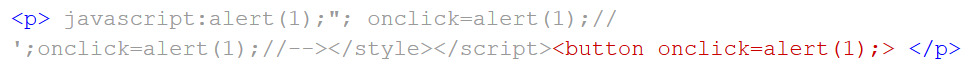
\includegraphics[width=\textwidth]{contents/images/PolyglottSingleExample}
			\caption{XSS-Polyglott: Funktion des Payload im HTML-Kontext}
			\label{fig:PolyglottSingleExample}
		\end{figure}
		
		\begin{figure}[htbp] 
			\centering
			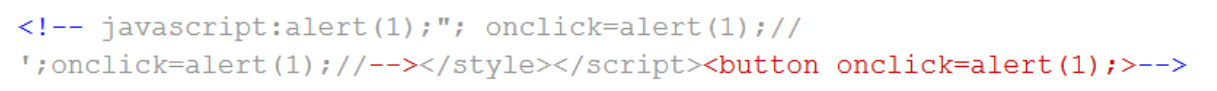
\includegraphics[width=\textwidth]{contents/images/PolyglottSingleExample2}
			\caption{XSS-Polyglott: Funktion des Payload im Kommentar-Kontext}
			\label{fig:PolyglottSingleExample2}
		\end{figure}
		
		Eine vollständige Darstellung, wie der Polyglott in den verschiedenen Kontexten funktioniert, ist in Anhang \ref{fig:PolyglottFullExample} dargestellt.
		
\subsection{\acl{HTML} 5 \& \acl{CSS} 3}
		Durch die neue Version 5 der \acl{HTML} sind viele Elemente und Events hinzugekommen, die die Verwendung von Multimedia-Inhalten vereinfachen. Diese bieten jedoch auch zusätzliche Ansatzpunkte, um XSS-Angriffe zu implementieren. 
		
		Mit HTML5 wurde auch \ac{CSS} in der dritten Version (\ac{CSS}3) vorgestellt. Mit Hilfe dieser Technik ist es Webentwicklern möglich, komplexe Animationen und visuelle Effekte nur unter Verwendung von \ac{CSS}3 abzubilden. Für Angreifer eröffnen sich durch die hierfür hinzugefügten JavaScript-Events weitere Möglichkeiten, eigenen Code einzuschleusen.		
		
		\noindent In den folgenden Beispielen (Quelltextbeispiele: \ref{HTML5CLOSINGEVENTSXSS} - \ref{CSS3ANIMATIONXSS}) ist exemplarisch aufgeführt, wie die neuen Elemente von HTML5 für \ac{XSS} genutzt werden können \cite{HTML5Sec2017}. 
		
\subsubsection{Events in schließenden Tags}
		
		Seit der neuen HTML-Version dürfen JavaScript-Events in schließenden HTML-Tags verwendet werden. Bisher wurden diese nicht ausgeführt.
		
\begin{lstlisting}[language=HTML,caption={XSS-Angriffe: Eventhandler in schließenden HTML-Tags},label=HTML5CLOSINGEVENTSXSS]
</a onmousemove="alert(1)">
\end{lstlisting}
		
\subsubsection{Neue HTML Tags}
		
		Neue Browser-Versionen können immer mehr mediale Inhalte darstellen und einbinden. Neben den hier aufgezählten MathML- und Video-Elementen können auch neue Audio- und Grafik-Elemente eingebunden werden.
		
\begin{lstlisting}[language=HTML,caption={XSS-Angriffe: Ausnutzen der MathML-Umgebung},label=HTML5MATHMLXSS]
<math href="javascript:alert(1)">CLICKME</math>
\end{lstlisting}
\begin{lstlisting}[language=HTML,caption={XSS-Angriffe: Ausnutzen des video-Tags},label=HTML5VIDEOXSS]
<video src=0 onerror="alert(1)">
<video poster=javascript:alert(1)//></video>
\end{lstlisting}
		
		Für IFrames ist das neue srcdoc-Attribut zum Einbinden lokaler HTML-Elemente auf dem Server eingefügt worden. Wie im Quelltext \ref{HTML5SRCDOCXSS} zu sehen ist, wird der Payload so kodiert, dass dieser vor dem Ausführen erst vom Browser interpretiert werden muss.
		
\begin{lstlisting}[language=HTML,caption={XSS-Angriffe: Ausnutzen der srcdoc-Eigenschaft von IFrames},label=HTML5SRCDOCXSS]
<iframe srcdoc="&lt;img src&equals;x:x onerror&equals;alert&lpar;1&rpar;&gt;" />
\end{lstlisting}
		
\subsubsection{Nutzen des autofocus-Tags}
		
		Das autofocus-Attribut soll bei Aufruf der Webseite den Cursor direkt in das erste Eingabefeld setzen. Dieses Attribut kann in Verbindung mit anderen Mechanismen, wie zum Beispiel dem Ausblenden von Elementen oder dem Scrollen der Webseite, JavaScript-Events auslösen.
		
\begin{lstlisting}[language=HTML,caption={XSS-Angriffe: Ausnutzen der autofocus-Eigenschaft},label=HTML5AUTOFOCUSXSS]
<!--Trigger: Leaving the input-->
<input onblur=alert(1) autofocus><input autofocus> 
<!--Trigger: Loading the website-->
<body onscroll=alert(1)><br><br><br>...<br><br><input autofocus>
\end{lstlisting}
		
\subsubsection{Angriffe mittels CSS-Animationen}
		
		Durch die Erweiterung von CSS können Animationen in der Auszeichnungssprache definiert werden. Unter Verwendung des Animations-Events können Payloads eingefügt werden.
		
\begin{lstlisting}[language=HTML,caption={XSS-Angriffe: Ausnutzen von CSS3-Animationen},label=CSS3ANIMATIONXSS]
<!--Auslöser: Laden der Webseite-->
<style>@keyframes x{}</style>
<div style="animation-name:x" onanimationstart="alert(1)"></div>
\end{lstlisting}